%%%%%%%%%%%%%%%%%%%%%%%%%%%%%%%%%%%%%%%%%%%%%%%%
%
% figures - nothing too special here 
%
%%%%%%%%%%%%%%%%%%%%%%%%%%%%%%%%%%%%%%%%%%%%%%%%
\chapter{Figures}


% BASIC EXAMPLE
%================

\begin{figure}[h!tb]
\centering

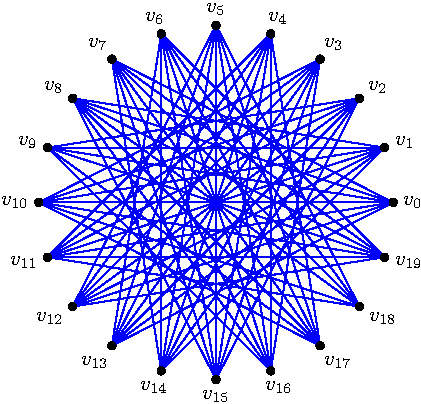
\includegraphics{figure} % not necessary to give extension - now you can shift between compiling to ps or to pdf without any problems
 
\caption[Figure caption in list of figures]{An example of the figure environment}

\end{figure}





\newpage





% SUBFIG EXAMPLE
%================
%
% usage: \subfloat[][caption]{...figure code...\label{label}}

The subfigures are Figures \subref{firstfigure}, \subref{secondfigure}, \subref{thirdfigure} and \subref{fourthfigure}.

\begin{figure}
\centering

\subfloat[][First subcaption.]{
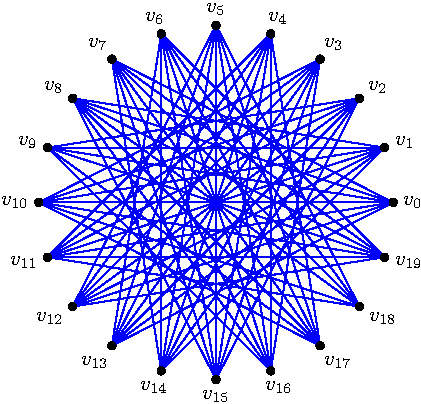
\includegraphics{figure}
\label{firstfigure}
}
\quad
\subfloat[][Second subcaption]{
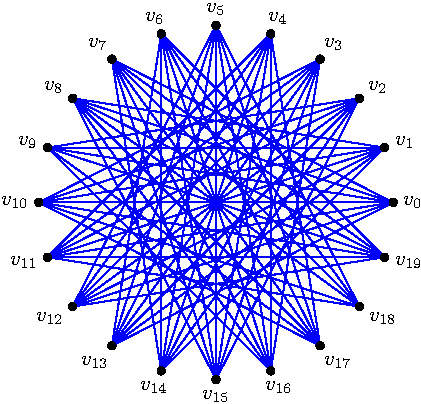
\includegraphics{figure}
\label{secondfigure}
}
\\
\subfloat[][Third subcaption]{
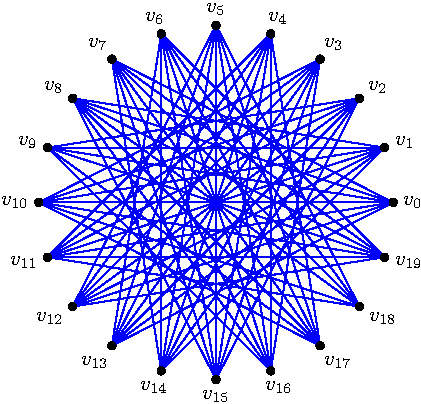
\includegraphics{figure}
\label{thirdfigure}
}
\quad
\subfloat[][Fourth subcaption]{
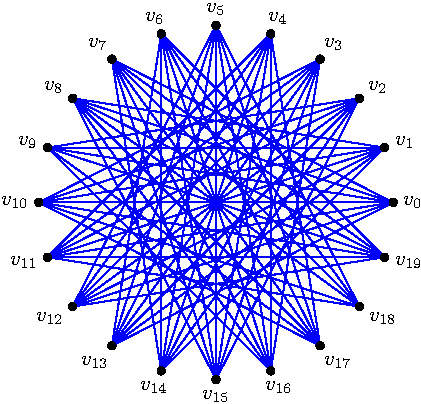
\includegraphics{figure}
\label{fourthfigure}
}
\caption{How to use the {\sf subfig} package.}
\label{thislabel}
\end{figure}
